\section{Method}

This section describes the Protective-Field Barrier (PFB) filter (4.2), the classical controllers beneath which it is placed (4.3) and a planned comparator filter (4.4).

\subsection{Overview}

Figure~\ref{fig:chain} shows the control chain of Eq. (4). The A$^{*}$ planner supplies a route on the map, which may omit obstacles. A classical controller proposes a nominal command $u_{\mathrm{nom}}$. The PFB filter replaces it by the closest command that keeps every valid scan return outside the protective field of the regime the robot will be in. The certified layer then passes this command or stops the robot, and the actuation limits (axis box, wheel-speed budget, acceleration limiter) apply last. With the filter disabled, $\mathcal{P}$ is the identity, so a controller without it is exactly the unfiltered controller. Every comparison in this paper differs in one respect: whether the filter sits between the controller and the certified layer.

\begin{figure}[t]
\centering
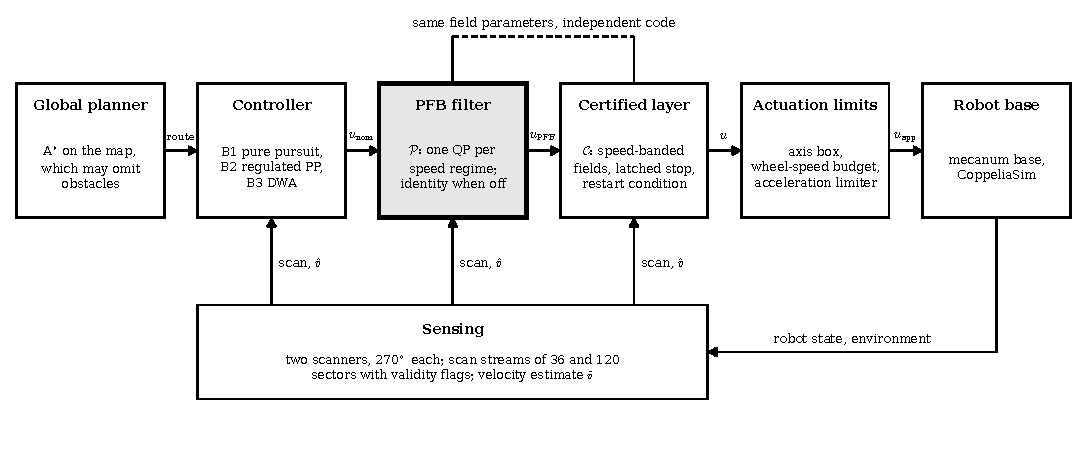
\includegraphics[width=\linewidth]{fig1_architecture.pdf}
\caption{Control chain of the proposed system. A global A$^*$ planner supplies a route on a map that omits some obstacles. A classical controller (B1, B2 or B3) maps the scan, the route lookahead and the goal to a nominal velocity command $u_{\mathrm{nom}}$. The Protective-Field Barrier (PFB) replaces $u_{\mathrm{nom}}$ by the closest command that keeps every valid scan return outside the protective field it will be in, and the certified layer then passes this command or applies a latched stop. The command $u$ drives the robot base in the simulator, whose state is read by the sensing block. The PFB and the certified layer use the same field parameters but independent code. With the filter switched off, the PFB is the identity. The shaded block is the proposed filter, $\mathcal{P}$ and $\mathcal{C}$ are the maps of Eq.~(4), and $u_{\mathrm{app}}$ is the command after the actuation limits.}
\label{fig:chain}
\end{figure}

\subsection{The Protective-Field Barrier filter}

\emph{Safe set.} The certified layer triggers when a valid scan point lies inside its field for the current band (1). The PFB takes the complement of that trigger region, with the discrete band fields replaced by a continuous protective field $\rho$ that depends on the command. Let $u = (v_x, v_y, \omega)$ be a candidate command and $\tau = \Delta t + \ell$ the prediction horizon, where $\ell = 0.05$ s is a lag allowance for the estimation delay. For the $i$-th valid scan return, let $r_i(u)$ and $\psi_i(u)$ be its range and bearing in the body frame after the robot has travelled at $u$ for $\tau$. The barrier row of return $i$ is

\begin{equation*}
g_i(u) = r_i(u) - \rho\big(\psi_i(u);\, \theta(u),\, W(u)\big) - \delta,
\tag{6}
\end{equation*}

and the candidate discrete-time condition (cf. (2) and (3)) is

\begin{equation*}
g_i(u) \ \ge\ (1 - \alpha \Delta t)\,\max\big(h_i^{\mathrm{now}},\, 0\big) \quad \text{for every valid return } i,
\tag{7}
\end{equation*}

where $h_i^{\mathrm{now}}$ is the same quantity at the current state. The function $\rho(\psi; \theta, W)$ is the distance from the robot to the boundary of the protective field along bearing $\psi$. The field is the footprint swept over the heading change reachable in $\tau$, extended along the heading $\theta(u)$ of the command by the distance travelled over the reach time plus the braking distance, $D(V) = V T + V^2 / (2 a_{\mathrm{brake}})$, and by margins. The heading $\theta(u)$ follows the command where it dominates the velocity estimate, and $W(u) = \max(|\hat\omega|, |\omega|)$ is the yaw rate for which the field is swept. The offset $\delta$ is the measured binning penalty of the scan at its upper bound (0.5 mm). Because the field is built from the same configuration as the certified layer but by independent code, the two cannot drift apart silently. The row has the discrete-time, beam-wise form of earlier LiDAR barrier filters~\cite{olayemi2026}. It differs from a constant-margin row in that the field depends on the speed and direction of the command and on the yaw rate. Figures~\ref{fig:fields} and~\ref{fig:step} show the fields and one filter step.

Taking the maximum with zero in (7) fixes the behaviour at a breached regime. If a return is already inside the field of the regime the robot would be in, the filter requires it to be clear after one step, and it never lets the robot enter a breached regime from outside. As stated in Section 3.3, $h_i$ is a candidate barrier whose validity is not established.

\emph{Assumptions and limits.} The condition (7) is evaluated over one prediction horizon $\tau = 0.10$ s, on a grid of five motion fractions of the predicted motion, with each row tightened by a margin so that the minimum over the grid bounds the minimum over the whole horizon. Satisfying it establishes compatibility with the modeled field over this horizon. It does not establish continuous-time exclusion from the field over the rest of the trajectory. Its effectiveness depends on the accuracy of the kinematic model, the validity of the range measurements, the control interval and the representation of the speed-band switching. Table~\ref{tab:field} lists the field model and the filter parameters, and Figure~\ref{fig:flowchart} summarises one decision of the filter. The emulated field reproduces the structure of a speed-banded, latching protective-field system, with the footprint swept along the braking segment plus margins. It is not the configuration of a specific commercial device. The independent certified layer therefore remains necessary and active.

\emph{Quadratic program.} For each speed regime of the certified layer (the at-rest field, or the band selected by the reachable speed), the filter solves

\begin{equation*}
\min_{u}\ (u - u_{\mathrm{nom}})^{\top}\, \mathrm{diag}(1, 1, \rho_{\mathrm{out}}^{2})\,(u - u_{\mathrm{nom}})
\quad \text{s.t. (7) for all } i,\ \ u \in \mathcal{U}_{\mathrm{adm}},\ \ \text{speed within the regime}.
\tag{8}
\end{equation*}

The weight $\rho_{\mathrm{out}} = 0.3374$ m, the outer radius of the footprint, converts a yaw rate into the speed of the footprint's outermost point, so that translation and rotation are penalised in the same units. The admissible set contains the mecanum wheel-speed polytope, the axis box, and the one-step envelope of the acceleration limiter. The rows (7) are nonlinear in $u$. They are linearised, with tangent planes in the translation and chords in the yaw rate, and each row more than 0.5 m from binding is left out of the QP. The true rows are checked at the solution with no tolerance, and one re-linearisation is allowed. The best feasible regime wins. A regime is infeasible when its QP has no solution, or when the true rows, checked at the solution with no tolerance, are violated after the allowed re-linearisation. If no regime is feasible, the filter issues the maximum-braking command, within the acceleration limiter, and labels the step infeasible; these steps are counted and reported. Braking is a fallback and not a regular control response. It does not guarantee that the predicted field constraint holds or that the certified layer will not trigger: the layer stays active and can still latch a stop on that step or the next.

\emph{Under the latch.} While the certified layer is latched, only a command that its restart condition could release passes: a creep that recedes from every point inside the at-rest field, or a twist whose own band field is clear. Otherwise the output is zero. The filter never removes or weakens the certified layer, which remains the backstop.

\emph{Gain.} The gain $\alpha$ is frozen at 1.0 s$^{-1}$ for every filtered controller. This is the lowest value of the grid searched on the tuning scenarios, and we do not claim it is optimal. The effect of $\alpha$ on the stops is reported as a sensitivity result (Section 6.3).

\emph{Cost.} The QP is solved with an interior-point method. In the validation runs on the final host, the 95th percentile of the filter's decision time was 47.1 to 48.4 ms, inside the 50 ms control period (Section 6.6).

\begin{table}[t]
\caption{Parameters of the modeled protective field and of the filter. The values are configured, and the band speeds are not measured quantities.}
\label{tab:field}
\centering
\small
\begin{tabular}{p{4.4cm}p{7.8cm}}
\toprule
Item & Value \\
\midrule
Control period $\Delta t$ & 0.05 s \\
Prediction horizon $\tau = \Delta t + \ell$ & 0.10 s, with a lag allowance $\ell = 0.05$ s \\
Rows checked over the horizon & five motion fractions $\{0, 0.25, 0.5, 0.75, 1\}$, each row tightened by 0.5 mm \\
Response time of the layer & 0.10 s (reach time 0.15 s with one control period) \\
Braking deceleration $a_{\mathrm{brake}}$ & 1.0 m/s$^2$ \\
Speed bands, top speeds & 0.10, 0.30 and 0.51 m/s, selected by the reachable speed $v + a_{\max} T$ capped by the axis box and the wheel budget \\
Field margins & 0.10 m ahead when moving; 0.05 m abeam when moving and all round at rest \\
Footprint & measured table; inscribed radius 0.209 m, outer radius 0.3374 m \\
Scan validity & a sector is valid only if its whole extent, from the footprint edge to 1.0 m beyond it, is seen; an invalid sector is an obstacle at the footprint boundary \\
Binning penalty $\delta$ & 0.5 mm \\
\bottomrule
\end{tabular}
\end{table}

\begin{figure}[t]
\centering
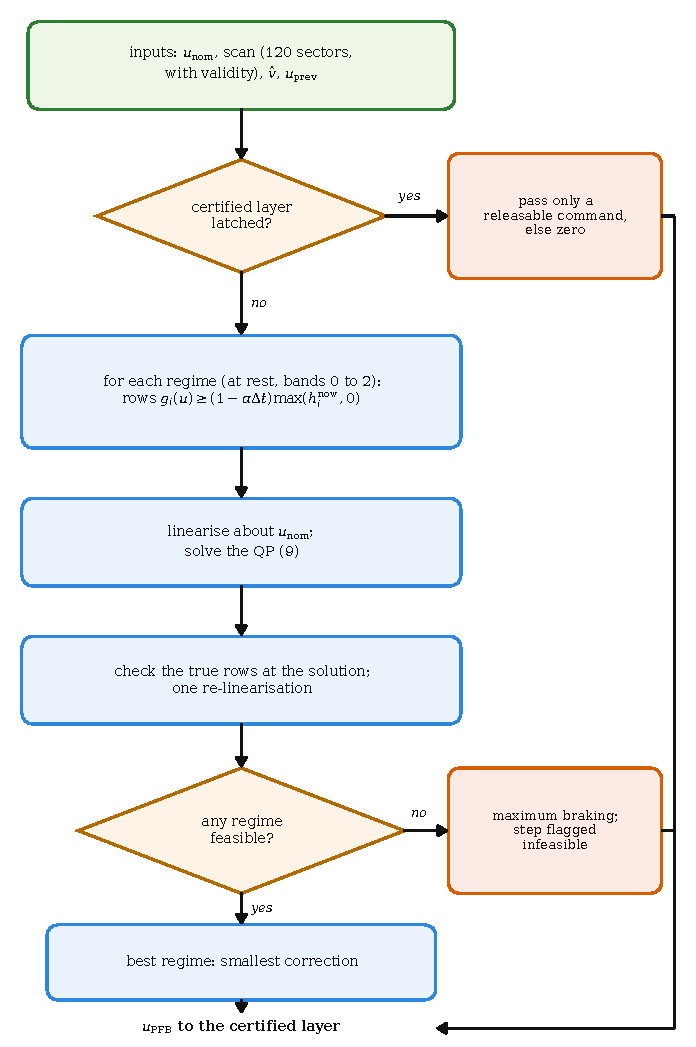
\includegraphics[width=0.62\linewidth]{fig_flowchart.pdf}
\caption{One decision of the PFB filter. While the certified layer is latched, only a command that its restart condition could release passes, and otherwise the output is zero. When it is not latched, the filter builds the barrier rows for each speed regime, linearises them about the nominal command, solves the QP (8), checks the true rows at the solution, and allows one re-linearisation. The regime with the smallest correction is used. If no regime is feasible, the filter commands maximum braking and flags the step. The output goes to the certified layer, which stays active.}
\label{fig:flowchart}
\end{figure}

\begin{figure}[t]
\centering
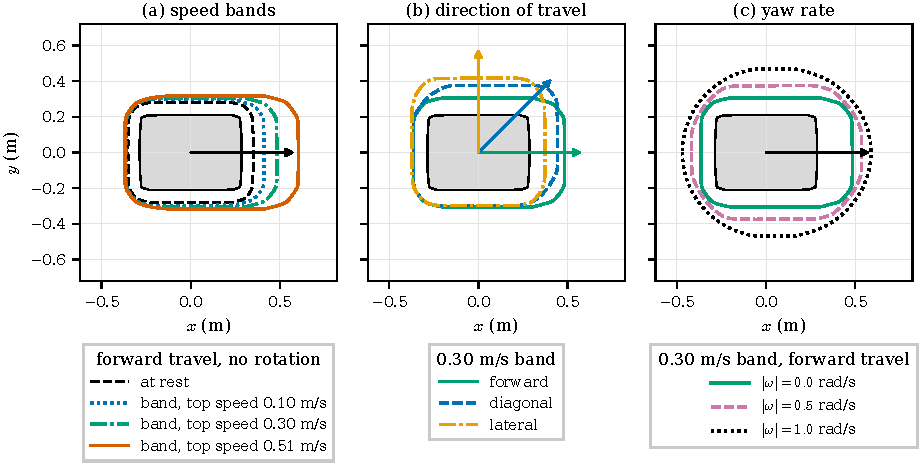
\includegraphics[width=\linewidth]{fig2_field_geometry.pdf}
\caption{Protective fields on the measured footprint (grey). Arrows give the direction of travel. (a) The at-rest field (dashed) and the fields of the three speed bands, with top speeds 0.10, 0.30 and 0.51~m/s, for forward travel without rotation. (b) The field of the 0.30~m/s band for forward, diagonal and lateral travel. (c) The field of the 0.30~m/s band for forward travel at yaw rates of 0, 0.5 and 1.0~rad/s.}
\label{fig:fields}
\end{figure}

\begin{figure}[t]
\centering
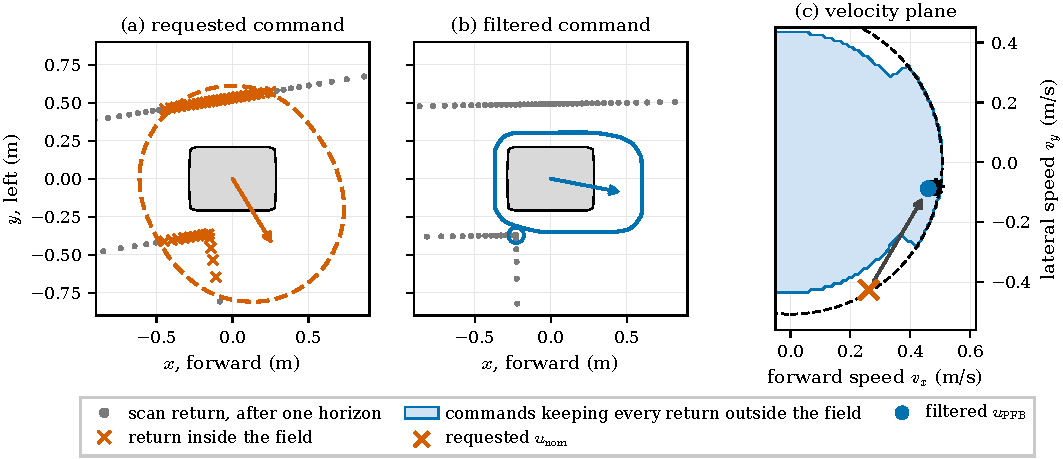
\includegraphics[width=\linewidth]{fig3_pfb_step.pdf}
\caption{One step of the PFB filter, for the step with the largest correction among those in which the requested command violates the field while the robot moves faster than 0.1~m/s. The requested command $u_{\mathrm{nom}}$ is illustrative and comes from a route-following command generator. The scenario is the first narrow-aisle scenario of the tuning set. (a) Robot frame: the protective field (dashed) of the speed regime that the filter selects, drawn for the requested command, and the scan returns as they would lie after one prediction horizon at that command. The crosses are the returns inside the field, each a violated barrier row. (b) The same for the filtered command $u_{\mathrm{PFB}}$: no return is inside its field, and the circle marks the binding return, the one with the least slack. (c) The plane of translational velocity at the filtered yaw rate. The shaded region contains the commands that keep every return outside the field, the dashed arc is the speed limit of the regime, and the dotted circle around the black square, the previously applied command, is the acceleration limiter's one-step envelope. The requested command (cross) lies outside the region, and the filtered command (dot) lies inside it. The requested yaw rate is $-1.45$~rad/s and the filtered yaw rate is approximately 0, so the cross shows the translational part of the requested command.}
\label{fig:step}
\end{figure}

\subsection{Classical controllers}

We evaluate three classical local controllers, each alone and with the PFB beneath. None accounts for the certified fields in its commands, so we call them field-blind. All three receive the same inputs: the route lookahead, the goal and the 120-sector scan stream, and no privileged information. All three run above the same certified layer and actuation limits, and all three use a speed cap derived from the map along the route and the same declared recovery after a latched stop, in which the controller waits a further 1.0 s after the layer's restart delay, then translates at 0.018 m/s for up to 0.30 m in the clearest of 72 body-frame directions, for up to five attempts per episode. Each controller is tuned alone, by the same protocol on the tuning scenarios (Section 5.3), and the filtered version keeps the tuned parameters unchanged.

\emph{B1, holonomic pure pursuit.} The controller steers toward the lookahead point on the route at a cruise speed, with a yaw gain and a slowdown near the goal. It does not use the scan, so it relies on the certified layer to stop it. Its tuned parameters are the cruise speed, yaw gain, goal slowdown and lookahead distance. \cite{coulter1992purepursuit}

\emph{B2, regulated pure pursuit.} The controller follows the route as pure pursuit does and, in the manner of the Nav2 regulated variant, reduces its speed with the curvature of the path and with the proximity of obstacles seen in the live scan. Its tuned parameters are the desired speed, the lookahead time and distance limits, the minimum turning radius, the proximity and approach distances, the minimum speeds and two gains. \cite{macenski2023rpp}

\emph{B3, holonomic dynamic window.} The controller samples commands reachable within one acceleration window and scores the short trajectories they produce for progress, heading and clearance. Its tuned parameters are the maximum speed, the window and simulation times, a safety margin and clearance cap, and three score weights. The first candidate takes the Nav2 DWB defaults. \cite{fox1997dwa}

In the tables, a controller with the filter beneath is written with a suffix, for example B3 + PFB.

\subsection{Planned comparator: a constant-margin beam filter}

To test whether the speed- and direction-dependent field is what removes stops, and not any beam-wise discrete-time barrier, we plan a comparator filter in the manner of the perception-aware filter of~\cite{olayemi2026}. Its field is the footprint's own extent plus one constant margin of 0.10~m, in every speed regime and for every heading and yaw rate of the command. It keeps the same discrete-time row form, the same gain, the same quadratic program and the same actuation limits, and it runs on the same hosts and beneath the same certified layer. The margin was fixed before the comparator was run, and it is not tuned on any set used to evaluate it. In the narrowest aisle it leaves 98.7~mm between the field and the wall for a centred robot. \tbd{the comparator has not been run}

